\documentclass[12pt,onesided]{amsart} 

%%%%%%%%%%%%%%%%%%%%%%%%%%%%%%%%%%%%%%%%%%%%%%%%%%
%%%%%%%%%%%%%%%%%%%% PREAMBLE %%%%%%%%%%%%%%%%%%%%
%%%%%%%%%%%%%%%%%%%%%%%%%%%%%%%%%%%%%%%%%%%%%%%%%%


% -------------------- defaults -------------------- %
% load lots o' packages

% layout control
\usepackage{geometry}
\geometry{verbose,tmargin=1.25in,bmargin=1.25in,lmargin=1.1in,rmargin=1.1in}
\usepackage[figuresright]{rotating}
\newenvironment{amssidewaysfigure}
  {\begin{sidewaysfigure}\vspace*{.8\textwidth}\begin{minipage}{\textheight}\centering}
  {\end{minipage}\end{sidewaysfigure}}
\usepackage{parallel}
\usepackage{parcolumns}

% math typesetting
\usepackage{array}
\usepackage{amsmath}
\usepackage{amssymb}
\usepackage{amsfonts}

\usepackage[%
decimalsymbol=.,
digitsep=fullstop
]{siunitx}

% to adapt caption style
\usepackage[font={small},labelfont=bf]{caption}

% references
\usepackage{natbib}
% \usepackage[natbib=true, style=authoryear]{biblatex}
% \bibliography{master.bib}

% footnotes at bottom
\usepackage[bottom]{footmisc}

% to change enumeration symbols begin{enumerate}[(a)]
\usepackage{enumerate}

% to make enumerations and itemizations within paragraphs or
% lines. f.i. begin{inparaenum} for (a) is (b) and (c)
\usepackage{paralist}

% to colorize links in document. See color specification below
\usepackage[x11names]{xcolor}

% load the hyper-references package and set document info
\usepackage[pdftex]{hyperref}

% graphics stuff
\usepackage{subfig}
\usepackage{graphicx}
\usepackage[space]{grffile} % allows us to specify directories that have spaces
\usepackage[section]{placeins} % prevents floats from moving past a \FloatBarrier or section
\usepackage{tikz}

% Spacing
\usepackage[doublespacing]{setspace}

% define clickable links and their colors
\hypersetup{
	unicode=false,          % non-Latin characters in Acrobat's bookmarks
	pdftoolbar=true,        % show Acrobat's toolbar?
	pdfmenubar=true,        % show Acrobat's menu?
	pdffitwindow=false,     % window fit to page when opened
	pdfstartview={FitH},    % fits the width of the page to the window
	pdfnewwindow=true,%
	pdfauthor={Minhas and Radford},%
	pdftitle={Enemy at the Gates},%
	colorlinks,%
	citecolor=black,%
	filecolor=black,%
	linkcolor=black,%
	urlcolor=RoyalBlue4%
	}
% -------------------------------------------------- %


% -------------------- title -------------------- %

\title[Enemy at the Gates]{Enemy at the Gates: Variation in Economic Growth from Civil Conflict}
\date{\today}

\author[Minhas]{Shahryar Minhas}
\address{Shahryar Minhas: Department of Political Science}
\curraddr{Duke University, Durham, NC, 27708, USA}
\email{shahryar.minhas@duke.edu}

\author[Radford]{Benjamin J. Radford}
\address{Benjamin J. Radford: Department of Political Science}
\curraddr{Duke University, Durham, NC, 27708, USA}
\email{benjamin.radford@duke.edu}


% \thanks{We are grateful for comments on earlier versions of this paper received at the 72$^{nd}$ annual Midwest Political Science Association Conference in Chicago, April 2-6 2014. }

% ----------------------------------------------- %


% -------------------- customizations -------------------- %

% easy commands for number propers
\makeatletter
\def\input@path{{/Users/janus829/Dropbox/Research/Rhodium/Graphics/}, {/Users/Ben/Dropbox/Rhodium/Graphics/}, {/Users/s7m/Dropbox/Research/Rhodium/Graphics/}, {C:/Users/Ben/Dropbox/Rhodium/Graphics}}
\makeatother
\graphicspath{{/Users/janus829/Dropbox/Research/Rhodium/Graphics/}, {/Users/Ben/Dropbox/Rhodium/Graphics/}, {/Users/s7m/Dropbox/Research/Rhodium/Graphics/}, {C:/Users/Ben/Dropbox/Rhodium/Graphics/}}

% -------------------------------------------------------- %


%%%%%%%%%%%%%%%%%%%%%%%%%%%%%%%%%%%%%%%%%%%%%%%%%%
%%%%%%%%%%%%%%%%%%%% DOCUMENT %%%%%%%%%%%%%%%%%%%%
%%%%%%%%%%%%%%%%%%%%%%%%%%%%%%%%%%%%%%%%%%%%%%%%%%

\doublespacing

\begin{document}
% Wordcount: 9814
\maketitle

\begin{abstract}
\singlespacing
% Within the conflict literature there has been much disagreement about the relationship between civil wars, natural resources, and state economic performance. We find that this disagreement results from not accounting for the spatial disaggregation of conflict events within a country.  Other recent work has suggested that the location of civil conflicts within a state can lead to disparate outcomes in terms of conflict duration, state response, and the probability of rebel victory.  Drawing on these two literatures, we develop a theory to explain the economic consequences of civil conflict.

% Our theoretical model states that the economic impacts of civil conflict is contingent on the conflict's location relative to major economic and labor resources within a state.

% We use subnational data on the spatial distribution of conflict, resources, and infrastructure to test the long-term impact of domestic conflict on state economic performance. To estimate the spatial distribution of conflict we use data from the PRIO Armed Conflict Location and Event Data and supplement this source with GDELT in more recent years. We combine the conflict location data with geospatial data on economic centers, natural resource locations, and infrastructure grids within the country to generate country-level spatial variables that approximate how far each conflict is from centers of interest for the government. We then use a hierarchical Bayesian model to estimate the effect of our spatially constructed variables on economic performance. By doing so, we are able to resolve some of the tensions in the literature regarding the relationship between economic performance and civil wars.

% Version submitted to MPSA:
Within the conflict literature there has been much disagreement about the relationship between civil wars, natural resources, and state economic performance. We find that this disagreement results from not accounting for the spatial disaggregation of conflict events within a country.

Our theoretical model states that the economic impact of civil conflict is contingent on the conflict's location relative to major economic and labor resources within a state.

We use subnational data on the spatial distribution of conflict, resources, and infrastructure to test the long-term impact of domestic conflict on state economic performance. To estimate the spatial distribution of conflict we use data from the PRIO Armed Conflict Location and Event Data. We combine the conflict location data with geospatial data on economic centers, natural resource locations, and infrastructure grids to generate spatial variables that approximate how far each conflict is from centers of interest. We then use a hierarchical Bayesian model to estimate the effect of the spatial variables on economic performance. By doing so, we are able to resolve some of the tensions in the literature regarding the relationship between economic performance and civil wars. 
\end{abstract}

\newpage
\newpage\setcounter{page}{1} 

%%%%% Appendix %%%%%

\newpage
\section*{Online Appendix}
\label{online_appendix}

\subsection{Illustrative Maps}
\label{maps}

FARC advocates a number of political and economic reforms and chooses targets strategically related to these objectives. Figure \ref{fig:colombiaMap} shows the spatial distribution of violence in Colombia from 1989 to 2008, where Bogot\'{a} is designated by a black diamond and major cities by black triangles. To determine the centroid locations of conflict we use the PRIO conflict site database developed by \citet{hallberg:2012}. 

\begin{figure}[ht]
	\centering
	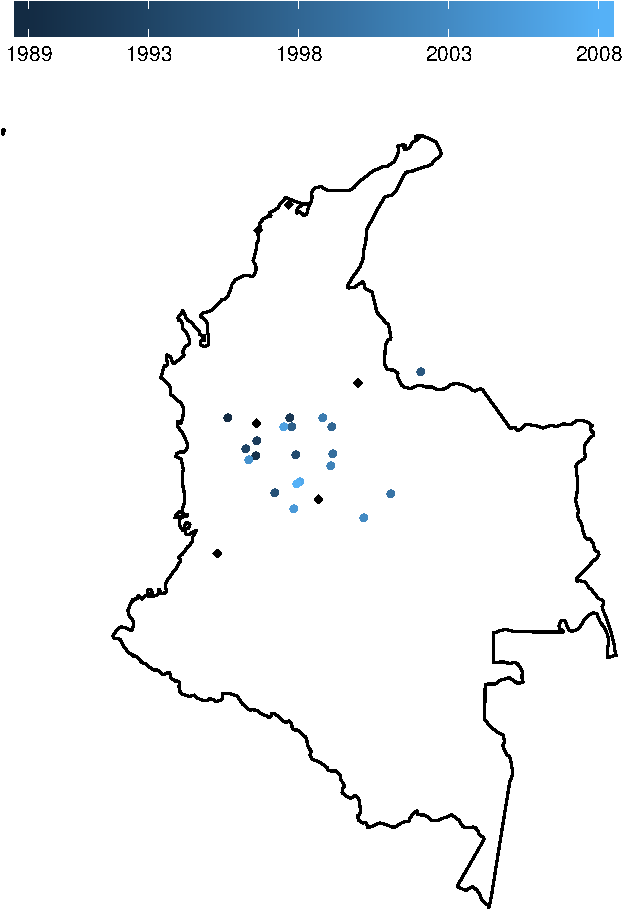
\includegraphics[width=.5\textwidth]{colombiaMap-crop}
	\caption{This map illustrates the geographic distribution of all conflict centroids in Colombia, according to the PRIO Conflict Site Dataset, and major cities from 1989 to 2008.}
	\label{fig:colombiaMap}
\end{figure}

In figure \ref{fig:indiaMap}, we show the geographic distribution of conflict in India from 1989 to 2007 again using the PRIO conflict site database. The story from this map is clearly quite stark from that of Colombia. Whereas in Colombia conflict had come right to the gates of major cities, in India conflict has been primarily confined to the periphery.

\begin{figure}[ht]
	\centering
	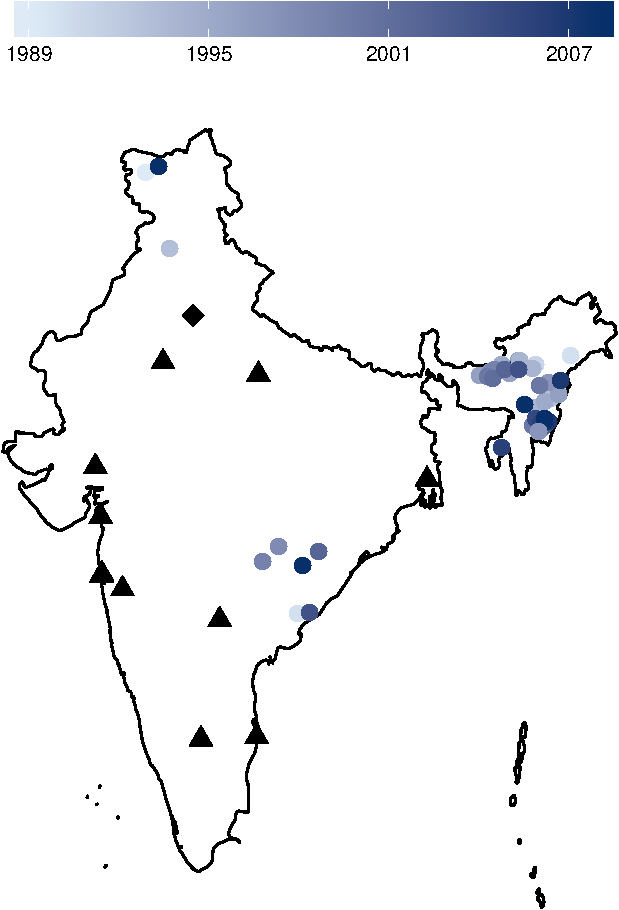
\includegraphics[width=.5\textwidth]{indiaMap-crop}
	\caption{This map illustrates the geographic distribution of all conflict centroids in India, according to the PRIO Conflict Site Dataset, and major cities from 1989 to 2007. }
	\label{fig:indiaMap}
\end{figure}

\newpage
\subsection{ACLED Analysis}
\label{acled}

The Armed Conflict Location and Event Dataset provides an alternative source of information on the subnational spatial distribution of armed conflict \citep{raleigh:linke:etal:2010}. This dataset is, at the time of writing, limited to Africa and therefore was not selected for the primary analysis presented in the text. It does, however, offer us a valuable opportunity to validate our results. Here, we have replicated the primary model described in Section~\ref{empirics}.

In order to match our existing data structure, it was necessary to aggregate the ACLED data to the country-year level. We did this by first subsetting ACLED to the years 1989-2008 and then selecting only conflict sites with at least 25 fatalities in each given year. The 25 fatalities threshold is intended to mirror the PRIO coding criteria and to prevent very low-fatality events from biasing our estimates of conflict location toward high-population areas. Covariates created with PRIO but unavailable in ACLED are omitted. The analysis procedure then continues as described in Section~\ref{empirics}: the minimum distance measure is calculated as the natural logarithm of the average distance in kilometers from any conflict site to the nearest major city (or capital). The results are presented in Table~\ref{tab:acledRegResults} below. 

When utilizing this alternative dataset we again find significant support for the argument that conflicts more proximate to urban centers have a greater adverse effect on economic growth than those farther away. Additionally, if we switched to a fixed effects framework, such as the one described in the previous appendix section, we still find significant support for the hypotheses laid out in our paper.

\begin{table}[!htbp] \centering 
  \caption{Random effects regression using ACLED.} 
  \label{tab:acledRegResults} 
\footnotesize{
\begin{tabular}{@{\extracolsep{5pt}}lcc} 
\\[-1.8ex]\hline 
\hline \\[-1.8ex] 
 & \multicolumn{2}{c}{\textit{Dependent variable:}} \\ 
\cline{2-3} 
\\[-1.8ex] & \multicolumn{2}{c}{$\% \Delta GDP_{t}$} \\ 
\\[-1.8ex] & (1) & (2)\\ 
\hline \\[-1.8ex] 
 Ln(Min. City Dist.)$_{t-1}$ & 0.585$^{**}$ &  \\ 
  & (0.254) &  \\ 
  & & \\ 
 Ln(Min. Cap. Dist.)$_{t-1}$ &  & 0.660$^{**}$ \\ 
  &  & (0.259) \\ 
  & & \\ 
 Number of conflicts$_{t-1}$ & 9.091$^{***}$ & 9.291$^{***}$ \\ 
  & (1.834) & (1.832) \\ 
  & & \\ 
 Ln(Inflation)$_{t-1}$ & 1.167 & 0.921 \\ 
  & (0.851) & (0.815) \\ 
  & & \\ 
 Democracy$_{t-1}$ & 0.147 & 0.116 \\ 
  & (0.217) & (0.217) \\ 
  & & \\ 
 Resource Rents/GDP$_{t-1}$ & $-$0.0001 & 0.004 \\ 
  & (0.048) & (0.048) \\ 
  & & \\ 
 World GDP Growth$_{t}$ & 1.034$^{**}$ & 0.877$^{**}$ \\ 
  & (0.442) & (0.439) \\ 
  & & \\ 
 Intercept & $-$19.308$^{***}$ & $-$18.398$^{***}$ \\ 
  & (5.477) & (5.252) \\ 
  & & \\ 
\hline \\[-1.8ex] 
Countries & 22 & 22  \\ 
Observations & 101 & 101 \\ 
\hline 
\hline \\[-1.8ex] 
\textit{Note:}  & \multicolumn{1}{l}{$^{*}$p$<$0.1; $^{**}$p$<$0.05; $^{***}$p$<$0.01} \\ 
\end{tabular} 
}
\end{table} 
\FloatBarrier

\newpage
\subsection{Estimating Models Separately for High and Low Intensity Conflicts}

Here instead of treating conflict intensity as a control, we re-do our primary random effect regression models estimating the effect of distance on growth, but restricting to the civil conflicts coded as wars and then a separate model for civil conflicts coded as low intensity events. In both low intensity and high intensity cases we find that the conflict distance variables remain significant and in the expected direction, and the $\beta$ estimate of our distance variables is noticeably higher when using high intensity versus low intensity civil conflict cases. The results are presented in Table~\ref{tab:modHiLoIntensity} below.

\begin{table}[!htbp] \centering 
  \caption{Random effects regressions by PRIO intensity. } 
  \label{tab:modHiLoIntensity} 
\footnotesize{
\begin{tabular}{@{\extracolsep{5pt}}lcccc} 
\\[-1.8ex]\hline 
\hline \\[-1.8ex] 
 & \multicolumn{4}{c}{\textit{Dependent variable:}} \\ 
\cline{2-5} 
\\[-1.8ex] & \multicolumn{4}{c}{$\% \Delta GDP_{t}$} \\ 
\\[-1.8ex] & (Low Intensity) & (High Intensity) & (Low Intensity) & (High Intensity)\\ 
\hline \\[-1.8ex] 
 Ln(Min. City Dist.)$_{t-1}$ & 1.163$^{***}$ & 2.281$^{**}$ &  &  \\ 
  & (0.409) & (1.130) &  &  \\ 
  & & & & \\ 
 Ln(Min. Cap. Dist.)$_{t-1}$ &  &  & 1.009$^{***}$ & 2.884$^{***}$ \\ 
  &  &  & (0.385) & (1.104) \\ 
  & & & & \\ 
 Duration$_{t-1}$ & 0.151$^{***}$ & 0.227$^{**}$ & 0.153$^{***}$ & 0.204$^{**}$ \\ 
  & (0.035) & (0.091) & (0.035) & (0.090) \\ 
  & & & & \\ 
 Area$_{t-1}$ & $-$3.794$^{***}$ & $-$8.995$^{***}$ & $-$3.603$^{***}$ & $-$7.606$^{***}$ \\ 
  & (1.345) & (2.636) & (1.366) & (2.703) \\ 
  & & & & \\ 
 Number of conflicts$_{t-1}$ & 1.367$^{**}$ & 1.262 & 1.332$^{**}$ & 1.406 \\ 
  & (0.573) & (3.599) & (0.573) & (3.556) \\ 
  & & & & \\ 
 Upper Income & 2.176 & $-$1.637 & 1.741 & $-$0.390 \\ 
  & (2.342) & (9.430) & (2.300) & (9.316) \\ 
  & & & & \\ 
 Ln(Inflation)$_{t-1}$ & $-$2.020$^{***}$ & $-$2.984$^{***}$ & $-$2.087$^{***}$ & $-$3.030$^{***}$ \\ 
  & (0.499) & (0.727) & (0.497) & (0.713) \\ 
  & & & & \\ 
 Democracy$_{t-1}$ & $-$0.051 & 0.117 & $-$0.073 & 0.118 \\ 
  & (0.089) & (0.214) & (0.089) & (0.211) \\ 
  & & & & \\ 
 Resource Rents/GDP$_{t-1}$ & 0.106$^{***}$ & $-$0.034 & 0.107$^{***}$ & $-$0.052 \\ 
  & (0.036) & (0.067) & (0.036) & (0.067) \\ 
  & & & & \\ 
 World GDP Growth$_{t}$ & 0.560$^{*}$ & 0.461 & 0.546$^{*}$ & 0.422 \\ 
  & (0.299) & (0.482) & (0.300) & (0.476) \\ 
  & & & & \\ 
 Intercept & $-$1.315 & $-$3.701 & $-$0.387 & $-$7.567 \\ 
  & (3.504) & (9.592) & (3.395) & (9.453) \\ 
  & & & & \\ 
\hline \\[-1.8ex] 
Countries & 66 & 30 & 66 & 30 \\ 
Observations & 403 & 131 & 403 & 131 \\ 
\hline 
\hline \\[-1.8ex] 
\textit{Note:}  & \multicolumn{4}{l}{$^{*}$p$<$0.1; $^{**}$p$<$0.05; $^{***}$p$<$0.01} \\ 
\end{tabular}
} 
\end{table} 
\FloatBarrier

\newpage
\subsection{Baseline Effect of Civil Conflict on Growth}

In Table \ref{tab:baseline} below, we show the fixed effects regression results for the model in which we utilize a full country year panel in order to define a baseline effect of civil war on economic growth. 

% Table created by stargazer v.5.1 by Marek Hlavac, Harvard University. E-mail: hlavac at fas.harvard.edu
% Date and time: Tue, Aug 25, 2015 - 15:53:07
\begin{table}[!htbp] \centering 
  \caption{This table shows the results of a country fixed effects regression in which we are utilizing a full country year dataset. } 
  \label{tab:baseline} 
\footnotesize{
\begin{tabular}{@{\extracolsep{5pt}}lc} 
\\[-1.8ex]\hline 
\hline \\[-1.8ex] 
 & \multicolumn{1}{c}{\textit{Dependent variable:}} \\ 
\cline{2-2} 
\\[-1.8ex] & $\% \Delta GDP_{t}$ \\ 
\hline \\[-1.8ex] 
 Civil War$_{t-1}$ & $-$2.568$^{***}$ \\ 
  & (0.502) \\ 
  & \\ 
 Ln(Inflation)$_{t-1}$ & $-$3.040$^{***}$ \\ 
  & (0.228) \\ 
  & \\ 
 Democracy$_{t-1}$ & 0.043 \\ 
  & (0.045) \\ 
  & \\ 
 Resource Rents/GDP$_{t-1}$ & 0.115$^{***}$ \\ 
  & (0.018) \\ 
  & \\ 
 World GDP Growth$_{t}$ & 0.673$^{***}$ \\ 
  & (0.081) \\ 
  & \\ 
\hline \\[-1.8ex] 
Countries & 160 \\
Observations & 3,002 \\ 
\hline 
\hline \\[-1.8ex] 
\textit{Note:}  & \multicolumn{1}{l}{$^{*}$p$<$0.1; $^{**}$p$<$0.05; $^{***}$p$<$0.01} \\ 
\end{tabular} 
}
\end{table} 
\FloatBarrier

\newpage
\subsection{Conflict Distance Models in Tabular Format}

Here we present the results of our models measuring the effect of conflict distance in a tabular format, results for distance from the capital city are shown in the first column of Table \ref{tab:capminDistMod} and for any major city in the second column.  

\begin{table}[!htbp] \centering 
  \caption{Tabular representation of coefficient plots shown in Figures 4a and 4b. }
  \label{tab:capminDistMod} 
\footnotesize{
\begin{tabular}{@{\extracolsep{5pt}}lcc} 
\\[-1.8ex]\hline 
\hline \\[-1.8ex] 
 & \multicolumn{2}{c}{\textit{Dependent variable:}} \\ 
\cline{2-3} 
\\[-1.8ex] & \multicolumn{2}{c}{$\% \Delta GDP_{t}$} \\ 
\\[-1.8ex] & (1) & (2) \\ 
\hline \\[-1.8ex] 
 Ln(Min. Cap. Dist.)$_{t-1}$ & 0.994$^{**}$ &  \\ 
  & (0.394) &  \\ 
  & & \\ 
 Ln(Min. City Dist.)$_{t-1}$ &  & 1.174$^{***}$ \\ 
  &  & (0.410) \\ 
  & & \\ 
 Intensity$_{t-1}$ & $-$1.146 & $-$1.190 \\ 
  & (0.971) & (0.970) \\ 
  & & \\ 
 Duration$_{t-1}$ & 0.144$^{***}$ & 0.143$^{***}$ \\ 
  & (0.037) & (0.037) \\ 
  & & \\ 
 Area$_{t-1}$ & $-$4.704$^{***}$ & $-$4.853$^{***}$ \\ 
  & (1.295) & (1.283) \\ 
  & & \\ 
 Number of conflicts$_{t-1}$ & 1.431$^{**}$ & 1.444$^{**}$ \\ 
  & (0.617) & (0.620) \\ 
  & & \\ 
 Upper Income & 0.696 & 1.051 \\ 
  & (2.691) & (2.720) \\ 
  & & \\ 
 Ln(Inflation)$_{t-1}$ & $-$2.639$^{***}$ & $-$2.564$^{***}$ \\ 
  & (0.469) & (0.471) \\ 
  & & \\ 
 Democracy$_{t-1}$ & $-$0.024 & $-$0.003 \\ 
  & (0.090) & (0.091) \\ 
  & & \\ 
 Resource Rents/GDP$_{t-1}$ & 0.072$^{**}$ & 0.072$^{**}$ \\ 
  & (0.036) & (0.036) \\ 
  & & \\ 
 World GDP Growth$_{t}$ & 0.543$^{**}$ & 0.554$^{**}$ \\ 
  & (0.272) & (0.271) \\ 
  & & \\ 
 Constant & 2.453 & 1.360 \\ 
  & (3.349) & (3.438) \\ 
  & & \\ 
\hline \\[-1.8ex] 
Countries & 69 & 69 \\
Observations & 505 & 505 \\ 
\hline 
\hline \\[-1.8ex] 
\textit{Note:}  & \multicolumn{2}{r}{$^{*}$p$<$0.1; $^{**}$p$<$0.05; $^{***}$p$<$0.01} \\ 
\end{tabular}
} 
\end{table} 

\FloatBarrier
\newpage


%%%%%%%%%%%%%%%%%%%%%%

\newpage

% \bibliographystyle{elsarticle-harv} 
\bibliographystyle{jpr}
\bibliography{master.bib}

\end{document} 